\subsection{Topics 5 \& 6: Operating System Fundamentals and Computational Complexity – Exercise Sheet [Solutions]}
\subsection*{Q\#1: Calculate number of times each word is printed:}
\begin{lstlisting}
int main() {
    fork();
    printf("Hello\n");
    fork();
    fork();
    printf("Beautiful\n");
    fork();
    fork();
    printf("World\n");
    return 0;
}
\end{lstlisting}
The number of times a word gets printed is equal to the number of processes created till that statement  
i.e. Total Number of \(Processes = 2^n\), where n is number of fork system calls executed so far.
In the example above, the word “Hello” gets printed 2 times, the word “Beautiful” is printed 8 times  
and the “World” is printed 32 times.

\subsection*{Q\#2: For First Come First Serve (FCFS) scheduling policy and using the given table, find the waiting  
time for each process and average waiting time in each of the following process arrival sequences:}

\begin{table}[htbp]
\begin{tabularx}{\textwidth}{| X | X |}
\hline
\textbf{Process} & \textbf{Burst time} \\
\hline
P1 & 10ms \\
\hline
P2 & 20ms \\
\hline
P3 & 14ms \\
\hline
P4 & 7ms \\
\hline
\end{tabularx}
\end{table}
\textbf{a.} P1, P2, P3, P4  \\
Waiting Time: P1: 0 ms , P2: 10 ms , P3: 30 ms , P4: 44 ms  \\
Average Waiting Time: 21 ms

\textbf{b.} P4, P2, P1, P3  \\
Waiting Time: P1: 27 ms , P2: 7 ms , P3: 37 ms , P4: 0 ms  \\
Average Waiting Time: 17.75 ms

\textbf{c.} P4, P3, P2, P1  \\
Waiting Time: P1: 41 ms , P2: 21 ms , P3: 7 ms , P4: 0 ms  \\
Average Waiting Time: 17.25 ms

\subsection*{Q\#3: For Shortest Remaining Time First Scheduling (SRTF) policy and using the given table, find the  
average waiting and average turnaround times in each of the following process orders:}

\begin{tabular}{lllll}
Process & Burst time & \multicolumn{3}{l}{Arrival Times} \\
& & a & b & c \\
P1 & 4 ms & 0 ms & 0 ms & 4 ms \\
P2 & 7 ms & 1 ms & 2 ms & 10 ms \\
P3 & 9 ms & 2 ms & 4 ms & 0 ms \\
P4 & 2 ms & 3 ms & 6 ms & 12 ms \\
\end{tabular}

\textbf{a.} For the given set of processes, here is the SRTF schedule:

\begin{table}[htbp]
\begin{tabularx}{\textwidth}{| X | X | X | X | X | X | X | X | X | X | X | X | X | X | X | X | X | X |X | X | X | X |}
\hline
P1&P1& P1 &P1 &P4 &P4 &P2 &P2 &P2 &P2 &P2 &P2 &P2 &P3 &P3 &P3 &P3 &P3 &P3 &P3 &P3 &P3\\
\hline
0 & 1 & 2 & 3 & 4 & 5 & 6 & 7 & 8 & 9 &10 &11 &12 &13 &14 &15 &16 &17 &18 &19 &20 &21\\
\hline
\end{tabularx}
\end{table}
Waiting Times: P1: 0 ms , P2: 5 ms , P3: 11 ms , P4: 1 ms  \\
Average Waiting Time: 4.25 ms  \\
Turnaround Times: P1: 4 ms , P2: 12 ms , P3: 20 ms , P4: 3 ms  \\
Average Turnaround Time: 9.75 ms

\textbf{b.} For the given set of processes, here is the SRTF schedule:

\begin{table}[htbp]
\begin{tabularx}{\textwidth}{| X | X | X | X | X | X | X | X | X | X | X | X | X | X | X | X | X | X |X | X | X | X |}
\hline
P1 & P1 & P1 & P1 & P2 & P2 & P4 & P4 & P2 & P2 & P2 & P2 & P2 & P3 & P3 & P3 & P3 & P3 & P3 & P3 & P3 & P3\\
\hline
0 & 1 & 2 & 3 & 4 & 5 & 6 & 7 & 8 & 9 &10 &11 &12 &13 &14 &15 &16 &17 &18 &19 &20 &21\\
\hline
\end{tabularx}
\end{table}

Waiting Times: P1: 0 ms , P2: 4 ms , P3: 9 ms , P4: 0 ms  \\
Average Waiting Time: 3.25 ms  \\
Turnaround Times: P1: 4 ms , P2: 11 ms , P3: 18 ms , P4: 2 ms  \\
Average Turnaround Time: 8.75 ms

\textbf{c.} For the given set of processes, here is the SRTF schedule:

\begin{table}[htbp]
\begin{tabularx}{\textwidth}{| X | X | X | X | X | X | X | X | X | X | X | X | X | X | X | X | X | X |X | X | X | X |}
\hline
P3 & P3 & P3 & P3 & P1 & P1 & P1 & P1 & P3 & P3 & P3 & P3 & P3 & P4 & P4 & P2 & P2 & P2 & P2 & P2 & P2 & P2\\
\hline
0 & 1 & 2 & 3 & 4 & 5 & 6 & 7 & 8 & 9 &10 &11 &12 &13 &14 &15 &16 &17 &18 &19 &20 &21\\
\hline
\end{tabularx}
\end{table}

Waiting Times: P1: 0 ms , P2: 5 ms , P3: 4 ms , P4: 1 ms  \\
Average Waiting Time: 2.50 ms  \\
Turnaround Times: P1: 4 ms , P2: 12 ms , P3: 13 ms , P4: 3 ms  \\
Average Turnaround Time: 8.00 ms

\subsection*{Q\#4: Consider the following table of processes and their associated arrival and running times.}

\begin{table}[htbp]
\begin{tabularx}{\textwidth}{| X | X | X |}
\hline
\textbf{Process ID} & \textbf{Arrival Time} & \textbf{Burst Time} \\
\hline
1 & 0 & 2 \\
\hline
2 & 1 & 6 \\
\hline
3 & 4 & 1 \\
\hline
4 & 7 & 4 \\
\hline
5 & 8 & 3 \\
\hline
\end{tabularx}
\end{table}

\textbf{a.} Show the scheduling order for these processes under 3 different policies: First Come First Serve  
(FCFS), Shortest-Remaining-Time-First (SRTF), Round-Robin (RR) with a quantum size = 1, by  
filling in the Gantt chart with ID of the process currently running in each time quantum. Assume  
that context switch overhead is 0 and that new RR processes are added to the head of the queue and  
new FCFS processes are added to the tail of the queue.\\

\begin{figure}[htp]
  \centering
  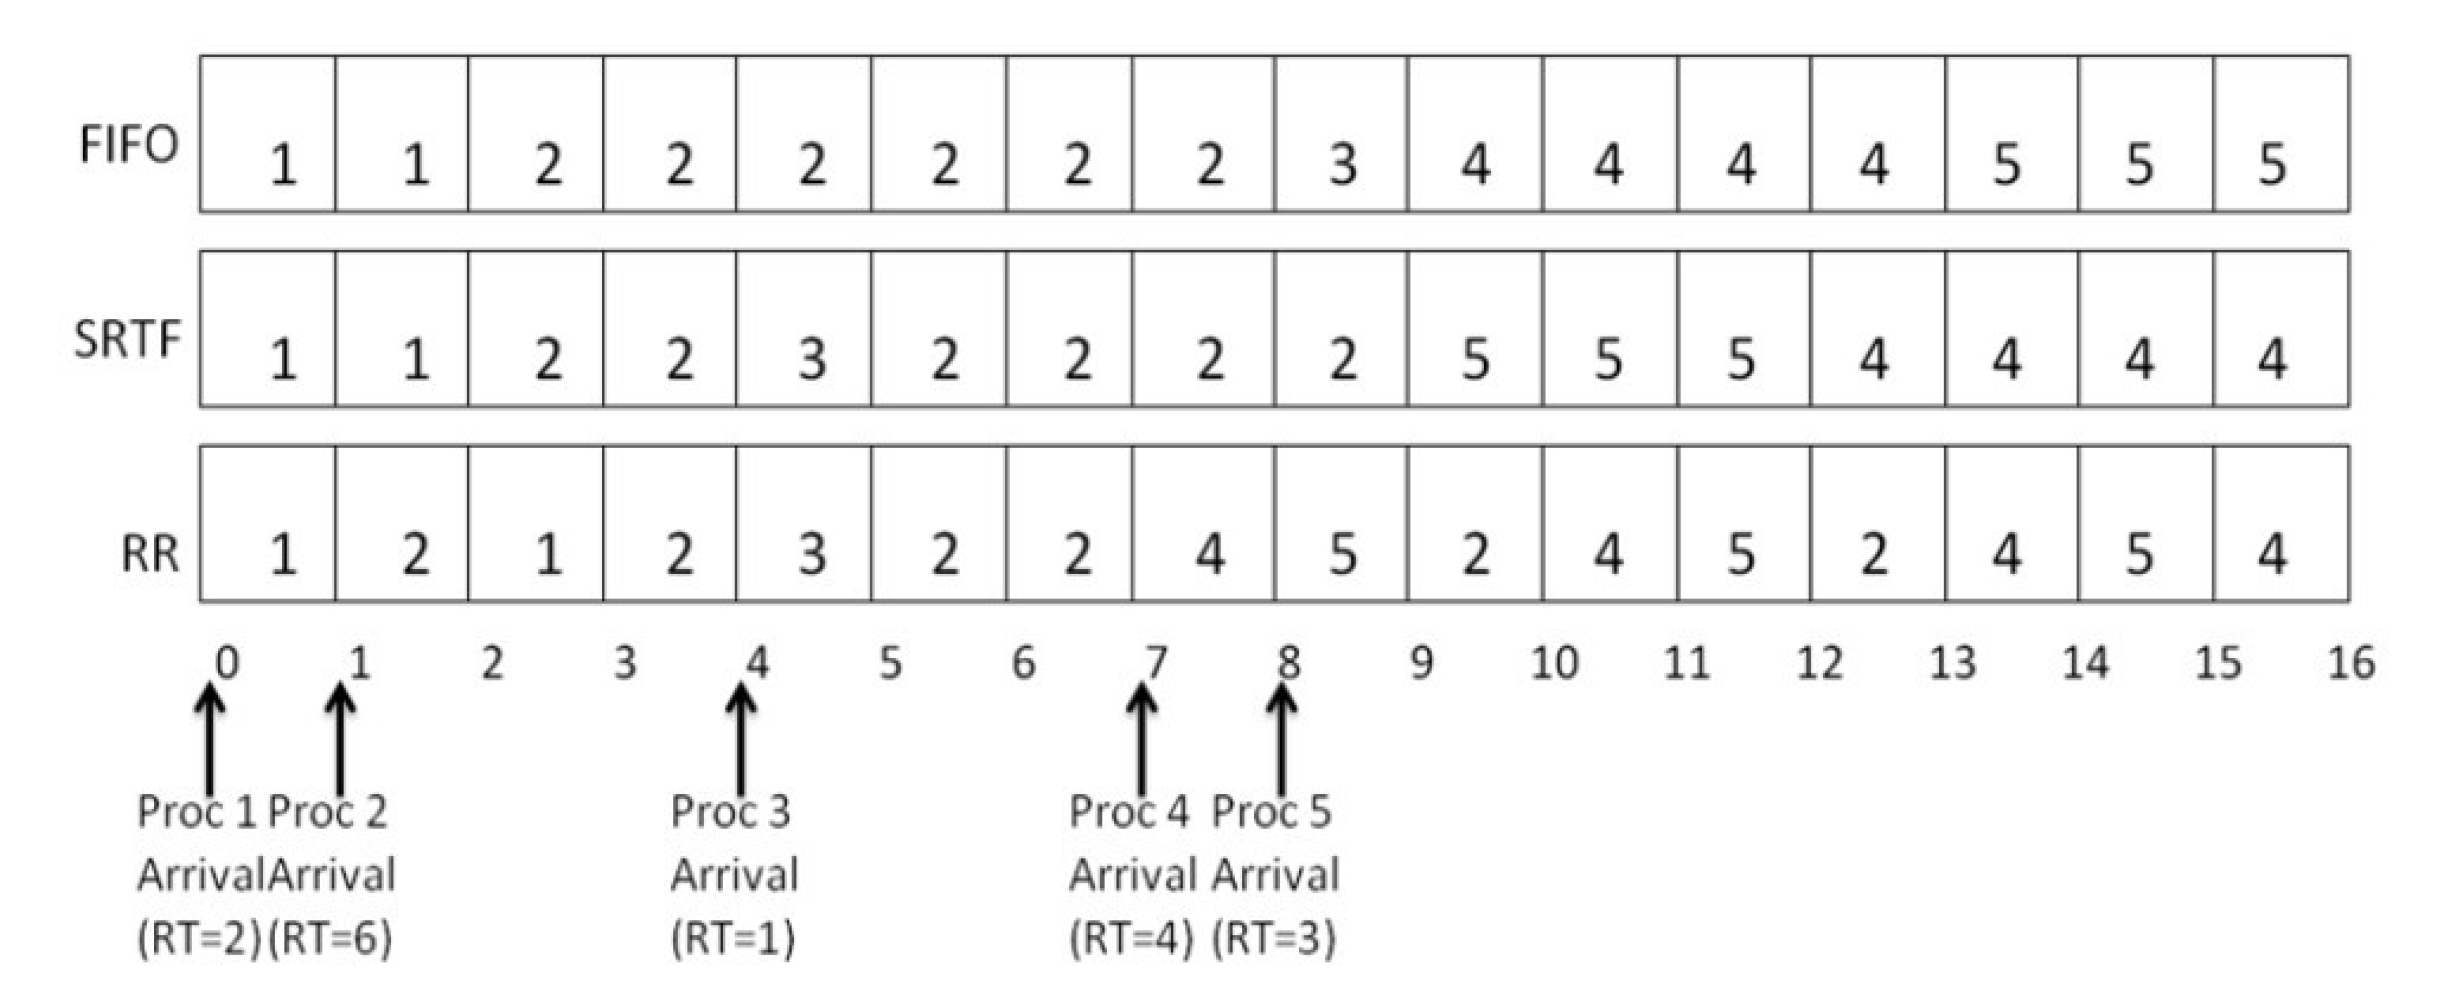
\includegraphics[width=15cm]{unit-22/figures/02.png}
  \caption*{currency}
\end{figure} 
\textbf{b.} Compute the response time for each process in each schedule above \& fill in the following table:

\begin{table}
\begin{tabularx}{\textwidth}{| X | X | X |X|X|X|}
\hline
       & \textbf{P1} & \textbf{P2} & \textbf{P3} & \textbf{P4} & \textbf{P5} \\
\hline
\textbf{FIFO} & \textcolor{blue}{0} & \textcolor{blue}{1} & \textcolor{blue}{4} & \textcolor{blue}{5} & \textcolor{blue}{5} \\
\hline
\textbf{SRTF} & \textcolor{blue}{0} & \textcolor{blue}{1} & \textcolor{blue}{0} & \textcolor{blue}{5} & \textcolor{blue}{1} \\
\hline
\textbf{RR}   & \textcolor{blue}{0} & \textcolor{blue}{0} & \textcolor{blue}{0} & \textcolor{blue}{0} & \textcolor{blue}{0} \\
\hline
\end{tabularx}
\end{table}

\subsection*{Q\#5: Consider the following fragment of Java-like code. Although this program does not really do anything, it is instructive to see how we can take actual code and analyze performance.}
\begin{lstlisting}
int a = 5;
int b = 6;
int c = 10; 
for (int i = 0; i < n; i++) {
   for (int j = 0; j < n; j++) {
      x = i * i;
      y = j * j; 
      z = i * j; 
   }
}

for (int k = 0; k < n; k++) {
   w = a * k + 45; 
   v = b * b; 
}

int d = 33; 
\end{lstlisting}

a) Formulate an expression to denote the overall execution time of this program considering that each Assignment Operation is treated as a unit of operation. \\ 
\textcolor{blue}{
The number  of  assignment  operations  is  the  sum of  four  terms.  The first  term is  the  constant  3, representing the three assignment statements at the start of the fragment. The second term is 3n², since there are three statements that are performed n² times due to the nested iteration. The third term is 2n, two  statements  iterated  n times.  Finally,  the  fourth  term is  the  constant  1,  representing  the  final assignment statement. This gives us T(n) = 3 + 3n² + 2n + 1 = 3n² + 2n + 4.
}\\
b) Identify the dominant term in this expression? \\ 
\textcolor{blue}{
By looking at the exponents, we can easily see that the 3n² term will be dominant.
}\\
c) What is the Worst Case Complexity of this program in terms of Big O notation?  \\
\textcolor{blue}{
Therefore this fragment of code is \(O(n^2)\). Please note that all of the other terms as well as the coefficient on the dominant term can be ignored as n grows larger.
}
\subsection*{Q\#6: What is the time complexity of the following code segments?}

(a)
\begin{verbatim}
int a = 0, b = 0;
for (i = 0; i < 1000; i++) {
    a = a + rand();
}
for (j = 0; j < n; j++) {
    b = b + rand();
}
\end{verbatim}
O(n)

(b)
\begin{verbatim}
int a = 0;
for (i = 0; i < n; i++) {
    for (j = n; j > i; j--) {
        a = a + i + j;
    }
}
\end{verbatim}
O(n²)

(c)
\begin{verbatim}
int i, j, k = 0;
for (i = n / 2; i <= n; i++) {
    for (j = 2; j <= n; j = j * 2) {
        k = k + n / 2;
    }
}
\end{verbatim}
O(n log n)

(d)
\begin{verbatim}
int numberFound = 0;
for i = 0..(n-1)/2
   for j = 0..(n-1)/2
      if BinarySearch(A[i,j])
         numberFound = numberFound + 1
\end{verbatim}
O(n² log n)

\subsection*{Q\#7: A program you have developed has a fixed startup time and a main algorithm which you know is
\(O(n^3)\). You have tested the program with 1 data item, and it takes 10 ms to execute. With 100 data items
it takes 15 ms to run. Estimate how long (in ms) this algorithm will take for 400 items?}
\textcolor{blue}{
With 1 item it takes 10 ms. This means that it has a fixed startup cost of approximately 10 ms
(the time to process 1 item is negligible).
With n=100 it takes 15 ms: 10 ms startup time + 5 ms to process the 100 items.
We know that the main algorithm is \(O(n^3)\). Therefore, if we have 4 times as much data, we can estimate
that it will take 43 = 64 times as long to execute that part of the program + the fixed startup time.
Therefore, it will take 10 + 64*5 = 10 + 320 = 330 ms
(If we double the amount of data then we would increase the time 23 times = 8 times. If we doubled it
again, it will be 43 times = 64 times and so on)
}
An algorithm has a fixed startup time and runs in time \(O(n^3)\).  
When n = 1, it runs in 10ms.  
When n = 100, it runs in 15ms.  

Determine the runtime for n = 400.

Processing time increase factor: \((400/100)^3\) = 64  
Processing time: 5ms × 64 = 320ms  
Total time = 320ms + 10ms = 330ms

\subsection*{Q\#8: A program you have developed has a fixed startup time and a main algorithm which you know is
\(O(n^4)\). You have tested the program with 1 data item, and it takes 50 ms to execute. With 500 data items
it takes 270 ms to run. Estimate how long (in ms) this algorithm will take for 1500 data items?}

With 1 item it takes 50 ms. This is approx. the fixed cost of the algorithm.\\
With n=500 it takes 270 ms: 50 ms startup time + 220 ms to process the 500 items. \\
The main algorithm is \(O(n^4)\). Therefore, if we have 3 times as much data, we can estimate that it will take \(3^4\) = 81 times as long to execute that part of the program + the fixed startup time.
Therefore, it will take 50 + 81*220 = 50 + 17820 = 17,870 ms

An algorithm has a fixed startup time and runs in time \(O(n^4)\). \\ 
When n = 1, it runs in 50ms. \\ 
When n = 500, it runs in 270ms. \\  
Determine the runtime for n = 1500. \\
Growth factor = \((1500 / 500)^4\) = 81 \\ 
Processing time = 220ms × 81 = 17820ms \\ 
Total time = 17820ms + 50ms = 17870ms